\chapter{Planificación}

\section{Planificación temporal}

Desde la asignación del \acrshort{TFM}, en diciembre de 2017, me percaté que iba a ser realmente complicado alcanzar la primera convocatoria con la carga de trabajo que suponía el máster. Por lo que decidí tomarlo con calma y llegar a septiembre, pero tras finalizar el curso comencé la realización de mis prácticas, lo cual unido a lo extenuado que había acabado el año me impidió alcanzar el objetivo. 

En Octubre de 2017 comencé a trabajar, lo que supuso muchas horas libres menos al día y me llevó un tiempo adaptarme. Por lo que no fue hasta Febrero de 2018 cuando me lo empecé a tomar en serio. Teniendo en cuenta mi limitada disponibilidad horaria, que apenas me permitía dedicarle 1-2 horas entre diario, esbocé una planificación con el objeto de entregar el proyecto en Julio de 2018, dicha planificación inicial se recoge en la siguiente tabla.

\begin{table} [h!]
	\centering
	\begin{tabular}{l c c c}
		\hline
		\textbf{Tarea}            & \textbf{Inicio} & \textbf{Fin} & \textbf{Duración} \\ \hline\hline
		Investigación             & 19/02/2018      & 23/04/2018   & 8 semanas         \\ \hline
		Obtención de datos        & 23/04/2018      & 07/05/2018   & 2 semanas         \\ \hline
		Procesado de datos        & 07/05/2018      & 21/05/2018   & 2 semanas         \\ \hline
		Búsqueda básica           & 21/05/2018      & 04/06/2018   & 2 semanas         \\ \hline
		Búsqueda con bibliometría & 04/06/2018      & 02/07/2018   & 4 semanas         \\ \hline
		Refinamiento              & 02/07/2018      & 09/07/2018   & 1 semana          \\ \hline
	\end{tabular}
	\caption{Planificación inicial de tareas}
\end{table}

Desgraciadamente fui incapaz de alcanzar el objetivo de Julio, algunas vacaciones y asuntos personales me hicieron replanificar para llegar a esta convocatoria de Septiembre.

\section{Gestión de recursos}
En este apartado describiré brevemente los recursos utilizados para llevar a cabo este proyecto tiendo en cuenta personal, hardware y software.

\subsection{Personal}
El único recurso humano que ha contribuido a la realización del proyecto soy yo mismo, actuando como cada uno de los diversos roles que llevan acabo el proceso de desarrollo de un proyecto de estas características.

\subsection{Hardware}
Respecto al hardware utilizado para este \acrshort{TFM} solo he requerido mi ordenador portátil personal, cuyas características se destacan en la siguiente tabla:

\begin{table} [h!]
	\centering
	\begin{tabular}{c c}
		\hline
		     CPU       & Intel \textregistered  Core \texttrademark  i7-4700MQ CPU @ 2.40GHz x 8 \\
		     RAM       & 8 GB RAM DDR3                                                           \\
		Almacenamiento & HDD 750 GB (5400 RPM)                                                   \\ \hline
	\end{tabular}
	\caption{Especificaciones del equipo utilizado}
\end{table}

Esto ha bastado para el desarrollo, pero sería necesario conseguir un servidor para llegar a poner en producción el sistema. Tampoco sería necesario nada muy potente, ya que incluso en mi propio ordenador los tiempos empleados en la búsqueda son bastante aceptables.

\subsection{Software}
Se han empleado utilidades de software libre en la totalidad del proyecto. Para una enumeración de las mismas y su función primordial ver el apartado \nameref{ch:herramientas}.

\section{Presupuesto}

En este apartado haré una estimación a \textit{grosso} modo de los costes de llevar a cabo el proyecto si el objetivo fuera desarrollar un producto listo para explotación (no olvidemos que esto es un prototipo). 

A pesar de la dilatada planificación temporal, si se fuera a implementar este sistema la duración se reduciría drásticamente, al contar con una persona trabajando a tiempo completo. Estimo que en 2 meses a tiempo completo un desarrollador de mis características podría finalizar el proyecto holgadamente. Para ponerle un costo a esto estimaré un salario de 15€/hora brutos, lo que a jornada completa serían 2400 € brutos al mes, a mi juicio, un salario digno para un ingeniero con máster, desgraciadamente nada real. 

Respecto a los costes de hardware sería necesario un equipo para el desarrollo algo más potente que el utilizado, ya que en momentos puntuales la memoria de mi equipo se ha visto desbordada.
Por ello lo indicado sería un portátil con 16 GB de RAM y almacenamiento SSD de 256GB que puede rondar los 1000€ ahora mismo. Teniendo en cuenta que el periodo de amortización de un equipo de estas características ronda los 3 años y que la duración del proyecto sería 2 meses eso dejaría un coste de 55,55 €

Además sería necesario un servidor donde desplegar el sistema para su explotación. Hoy en día son pocos los proyectos que puedan requerir la compra de un servidor físico teniendo en cuenta las posibilidades que ofrece la computación en la nube y la variada oferta de la que se dispone. Por ello se contrataría una instancia en \textit{Amazon Web Services} de tipo \texttt{i3.xlarge} con 4 núcleos, 30 GB de RAM y 1 TB de SSD cuyos costes estimados mensuales son de 220 €.

Respecto al software a utilizar se apostaría por el software libre con licencias que permitan la comercialización como Apache2 o MIT, por lo que el coste estimado en Software es de 0€.

Si el proyecto se desarrollara en el ámbito académico, para ayudar a la labor investigadora de una universidad, seguramente no habría que considerar costes para usar datos de artículos, ya que alta probabilidad, la universidad en cuestión contará con licencias o acuerdos con editoriales científicas como Elsevier. En caso de querer desarrollar este sistema para su explotación económica los gastos editoriales podrían suponer un importante sobre coste que hiciera peligrar la viabilidad del proyecto.

Para esta estimación supondré que se desarrolla el proyecto en un ambiente académico obviando los gastos mencionados previamente. En la siguiente tabla se recogen los gastos requeridos para el desarrollo de este sistema (2 meses de proyecto), a esto habría que sumar 220€ por cada mes que se mantenga el sistema desplegado en concepto de costes de infraestructura.

\begin{table} [h!]
	\centering
	\begin{tabular}{| c | c |}
		\hline
		\textbf{Elemento}           & \textbf{Coste} \\ \hline
		Recursos humanos            & 4800€          \\
		Hardware para el desarrollo & 55,55€         \\
		Servidor                    & 440 €          \\
		Software                    & 0 €            \\
		Gastos editoriales          & 0 €            \\ \hline
		TOTAL                       & 5295,55 €      \\ \hline
	\end{tabular}
	\caption{Estimación de costes del proyecto}
\end{table}

\newpage

\section{Metodología de desarrollo}
\label{sc:metodologia}
Para desarrollar este proyecto se ha empleado una metodología ágil similar a \textit{\GLS{Scrum}} \glsrefentry{Scrum} pero algo más relajada. Es un modelo particular ya que yo mismo soy el desarrollador, el coordinador (rol del \textit{Scrum máster}) y la persona encargada de definir las tareas y evaluar el cumplimiento de las mismas (el \textit{Product owner}).

Me he decantado por este modelo ya que permite más flexibilidad al enfrentarse a problemas en entornos desconocidos, como es este proyecto. También ha influido mi experiencia personal ya que con esta metodología he llevado a cabo tanto mi \acrshort{TFG} como mis proyectos en el ámbito laboral. 

Se basa en la descomposición del proyecto completo en pequeños subproyectos o \textit{sprints}, en los que define de manera acotada las tareas y objetivos del mismo. Permitiendo el refinamiento iterativo del producto final así como el aprovechamiento del conocimiento obtenido a lo largo de los \textit{sprint} para mejorar los venideros. Al contrario que otros modelos de desarrollo clásicos que resultan más estáticos y rígidos.

Con el objetivo de almacenar y versionar todo el material producido en este proyecto he utilizado la plataforma \textit{GitHub} y el sistema de control de versiones \textit{git}. En concreto he creado el repositorio \url{https://github.com/AythaE/TFM}.

\newpage
Para seguir el progreso de cada uno de los \textit{sprints} del proyecto he utilizado los tableros que ofrece el propio \textit{GitHub projects} donde cada una de sus tareas o tarjetas corresponden con \textit{issues} como se puede ver en la siguiente imagen. 

\begin{figure}[h]
	
	\centering
	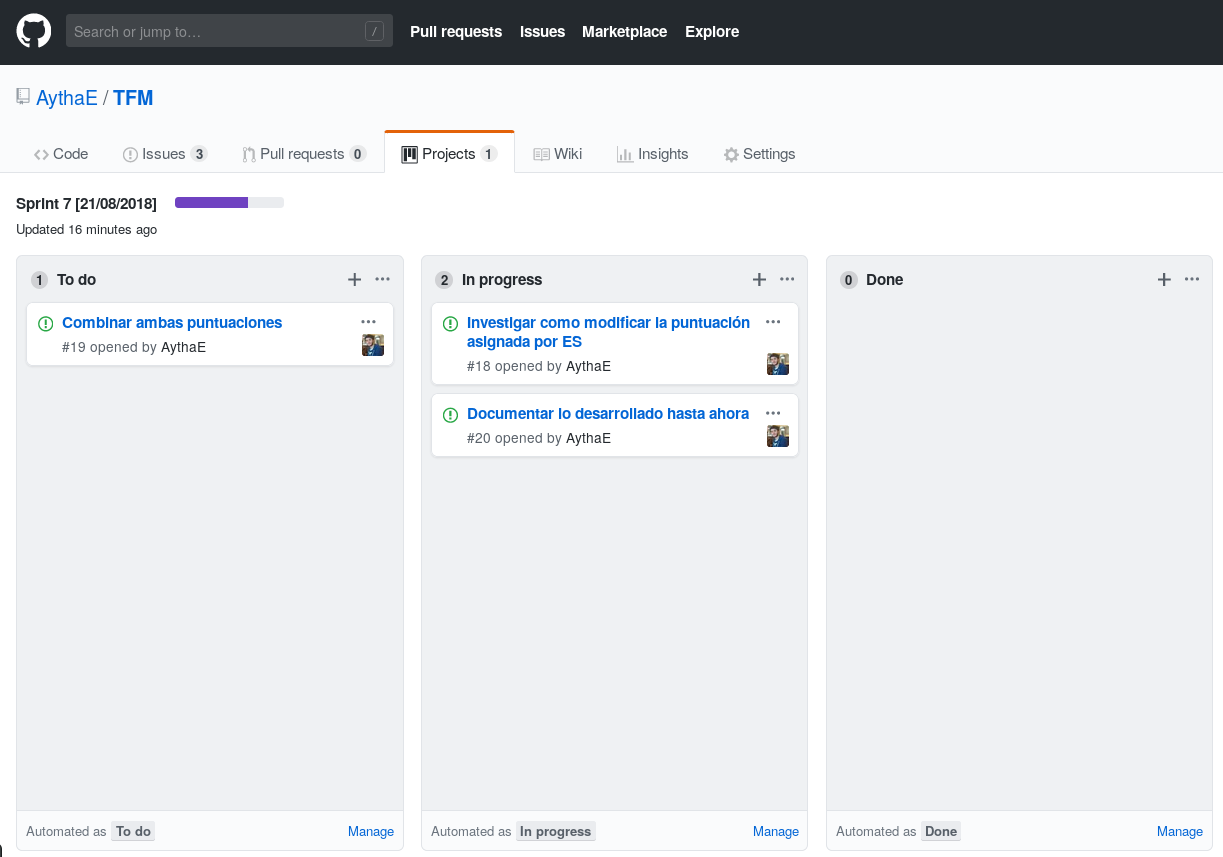
\includegraphics[width=\linewidth]{imagenes/ejemplo_tablero_sprint}
	\caption{Ejemplo de tablero de un \textit{sprint}}
	\label{fig:tableroSprint}
\end{figure}

Además de esto he utilizado un archivo \textit{Markdown} a modo de diario donde ir apuntando cosas interesantes según iban surgiendo, el estado actual de desarrollo o algunas tareas para completar próximamente, dicho fichero se llama \texttt{Diario.md}.
